\chapter{Implementation, Integration \& Test Plan}

This chapter of the \emph{Design Document} is devoted to explain the strategy that will be used while the \emph{Travlendar+} System will be develop, in order to define the procedure to follow when each components and each modules will be created, tested and integrated in the entire application.

\section{Integration Strategy}
The integration of the \emph{Travlendar+} components should start as soon as possible, in order to start the testing of both the single modules and the system's component.
But, before starting the integration phase, there are some precondition that should be satisfied:

\begin{itemize}

    \item The documents should be completed and written in a final version, both the \emph{RASD} and the \emph{Design Document}. Moreover, these documentation should be available to all the people involved in the project.
    
    \item The low-level units should be available to the \emph{Travlendar+} system. Indeed the \emph{Business Logic} layer, to work properly, needs to have a \emph{DBMS} ready and configured (so the \emph{Data} layer should be done), and some \emph{APIs} should be available, such as the map service, the transport service, the car-sharing and the bike-sharing services.
    
\end{itemize}

Once these preconditions are satisfied, when a component will be developed, it can be tested alone, and if it will work, then it can be integrated to the others components, in order to verify first the correct functionalities of the single module, and then that it works properly in the entire system.

The implementation should start with the elementary component of the \emph{Business Logic} layer, in this way the testing will be focused on the main, and most important, logic features. Indeed, the first components to develop are:

\begin{enumerate}
    \item Core Entities, in order to have the correct data structures.
    \item Access Data Manager, in this way the system can interact easily with a database.
    \item Scheduler, the main function of the \emph{Business Logic} layer, that will be developed in the following order:
    \begin{enumerate}
        \item Cost Evaluator, component used to check the goodness of a travel or a schedule.
        \item Day Scheduler, used to know if the algorithm works properly.
        \item Week Scheduler, used to test if the application can divide properly tasks through various days.
    \end{enumerate}
    \item General Preferences Manager, that will interact with the scheduler to set up the user's preferences in a correct way.
    \item FixedTask Fetcher, that should take various tasks to give them to the scheduler module
\end{enumerate}

After the development of the \emph{Business Logic} layer, the focus will be moved on the \emph{Presenter Layer}, in order to start the testing of the communication as soon as possible. Moreover, after the implementation and the integration of the \emph{Presenter Layer}, the Application Server can be set up to start its work.

Then the Application Server should interact with the internal Web Server, so the next move will be the development of the Application Façade layer, necessary to test the communication with the clients.
In parallel, the clients can be developed, so the entire communication part of the \emph{Travlendar+} application can be tested.

Here is detailed the diagram that shows the testing dependencies. As a notation, the arrows that goes from a component A to a component B means that the component A should be done before the component B in order to integrate and test properly the modules.

\begin{figure}[H]
    \centering
    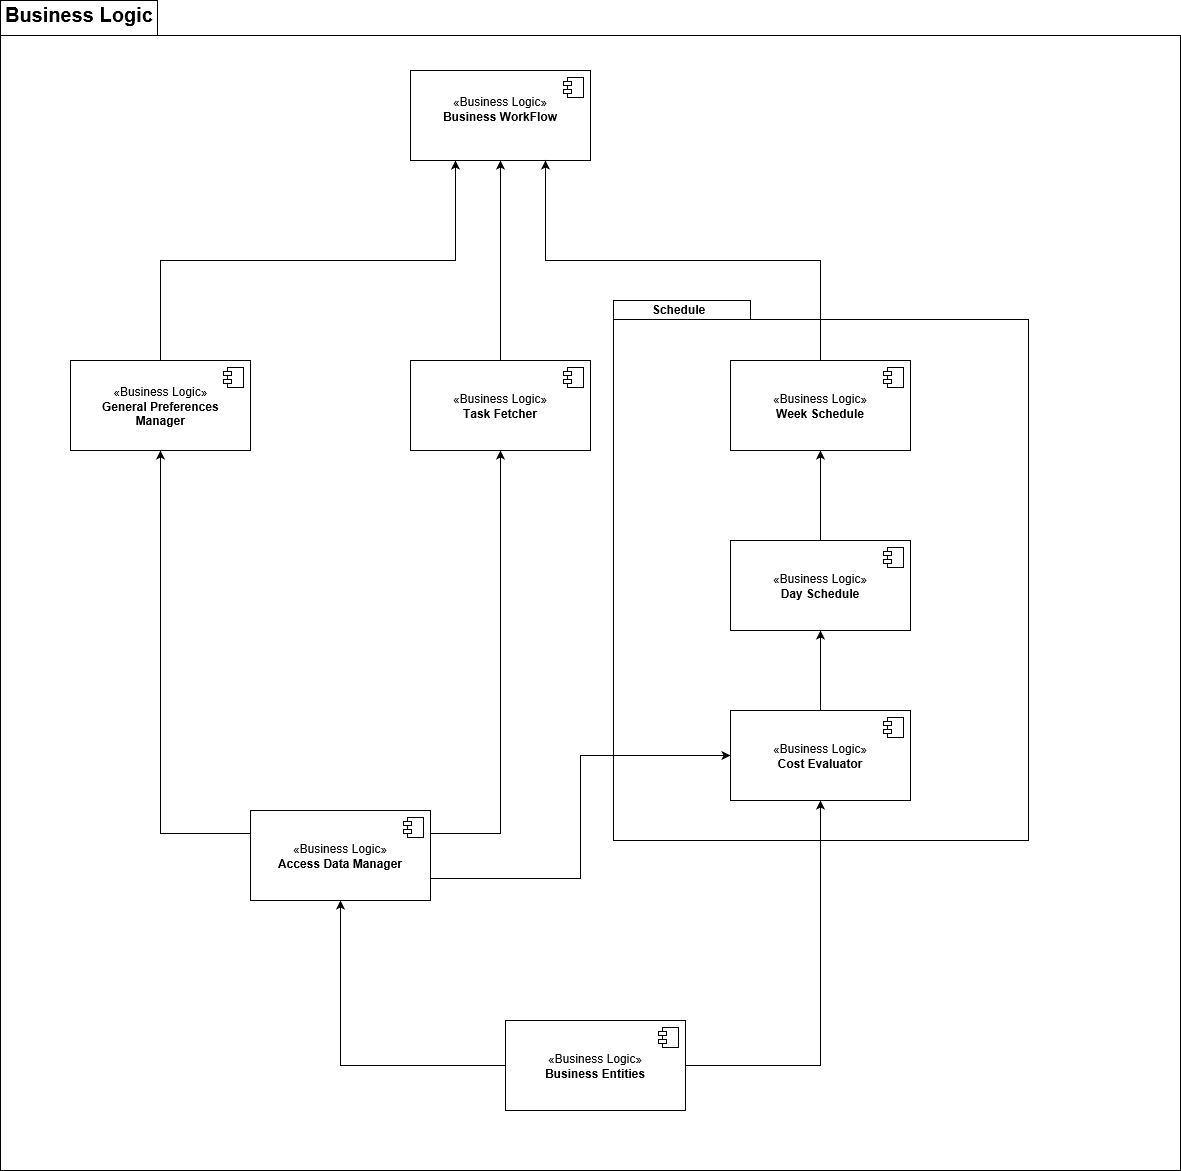
\includegraphics[scale=0.35]{Pictures/ImplementationDiagram/IntegrationDiagram.png}
    \caption{\emph{Travlendar+} integration, implementation and testing diagram}
\end{figure}

\section{Testing Description}

\renewcommand{\arraystretch}{1.9}

\subsection*{Login System}

\begin{table}[H]
    \centering
    \begin{tabular}{p{4.55cm} p{7cm}}
        
        \hline
        
        \textbf{Test ID}                & T1 \\
        
        \hline
        
        \textbf{Involved Components}    & Application Façade, Message Transmitter, Message Receiver, Business                                          WorkFlow, DBMS\\
        
        \hline
        
        \textbf{Input Specification}    & User's email and password\\
        
        \hline
        
        \textbf{Output Specification}   & System should check if both email and password are correct\\
        
        \hline
        
        \textbf{Exception}              & Either email or password are unvalid, so the system should show to the                                       user an error page\\
        
        \hline
        
        \textbf{Description}            & The system should be able to log in a user, by the verification of his                                      email and password. This procedure is done by receiving a message in the web server, send it to the Application server through the \emph{Message Receiver} component, analyzed by the \emph{Business WorkFlow} component and the \emph{DBMS} and then accept or discard, by send back a page through the Presenter's \emph{Message Transmitter} component\\
        
        \hline
        
        \textbf{Environmental needs}    & \\
        
        \hline
        
    \end{tabular}
    \caption{Testing Description of Login system}
\end{table}



\subsection*{Sign Up System}

\begin{table}[H]
    \centering
    \begin{tabular}{p{4.55cm} p{7cm}}
        
        \hline
        
        \textbf{Test ID}                & T2 \\
        
        \hline
        
        \textbf{Involved Components}    & Application Façade, Message Transmitter, Message Receiver, Business                                          WorkFlow, DBMS\\
        
        \hline
        
        \textbf{Input Specification}    & User's first name, last name, email, user residence and password\\
        
        \hline
        
        \textbf{Output Specification}   & System should add the user to the internal database, and send back an email to him with a summary of the operation done\\
        
        \hline
        
        \textbf{Exception}              & User enters a mail that is already registered in the system. So the system send back an error page and it doesn't register the user\\
        
        \hline
        
        \textbf{Description}            & The user send his information required by the system to save him in the DBMS. This message goes from the client to the Application Server, which thanks to the \emph{Business Logic} module can check the correctness of the information, and, if there aren't errors, store the user and give him an account\\
        
        \hline
        
        \textbf{Environmental needs}    & \\
        
        \hline
        
    \end{tabular}
    \caption{Testing Description of Sign Up system}
\end{table}



\subsection*{Add FixedTask System}

\begin{table}[H]
    \centering
    \begin{tabular}{p{4.55cm} p{7cm}}
        
        \hline
        
        \textbf{Test ID}                & T3 \\
        
        \hline
        
        \textbf{Involved Components}    & Application Façade, Message Transmitter, Message Receiver, Business                                          WorkFlow, Scheduler, DBMS\\
        
        \hline
        
        \textbf{Input Specification}    & FixedTask's Information\\
        
        \hline
        
        \textbf{Output Specification}   & System should create a calendar with the new task inserted\\
        
        \hline
        
        \textbf{Exception}              & The newer task conflicts with some other older tasks, and the system cannot schedule a feasible solution for the new set of tasks. In some cases this situation can happen because the newer task is unreachable in a feasible time from the others tasks, according to the given constraints\\
        
        \hline
        
        \textbf{Description}            & The system should add the task to the DBMS system, and should schedule a feasible calendar with the newer task, according to the given time constraints, the travel constraints and the user's preferences\\
        \hline
        
        \textbf{Environmental needs}    & T1: the user should be logged in the system\\
        
        \hline
        
    \end{tabular}
    \caption{Testing Description of Add FixedTask System}
\end{table}




\subsection*{Remove FixedTask System}

\begin{table}[H]
    \centering
    \begin{tabular}{p{4.55cm} p{7cm}}
        
        \hline
        
        \textbf{Test ID}                & T4 \\
        
        \hline
        
        \textbf{Involved Components}    & Application Façade, Message Transmitter, Message Receiver, Business                                          WorkFlow, Scheduler, Access Data Manager, FixedTask Fetcher, DBMS\\
        
        \hline
        
        \textbf{Input Specification}    & FixedTask ID that will be removed\\
        
        \hline
        
        \textbf{Output Specification}   & System should remove the selected task\\
        
        \hline
        
        \textbf{Exception}              & The given FixedTask ID doesn't exist, so the system show an error page\\
        
        \hline
        
        \textbf{Description}            & The user specifies the task he wants to remove, then he sends this information to the system. At this point, the \emph{Business WorkFlow} components interacts with the \emph{Access Data Manager} to search the selected task and remove it. Finally, the system asks to the user if he wants to reschedule or not the calendar\\
        \hline
        
        \textbf{Environmental needs}    & T1: the user should be logged in the system\\
        
        \hline
        
    \end{tabular}
    \caption{Testing Description of Remove FixedTask System}
\end{table}




\subsection*{Modify FixedTask System}

\begin{table}[H]
    \centering
    \begin{tabular}{p{4.55cm} p{7cm}}
        
        \hline
        
        \textbf{Test ID}                & T5 \\
        
        \hline
        
        \textbf{Involved Components}    & Application Façade, Message Transmitter, Message Receiver, Business                                          WorkFlow, Scheduler, Access Data Manager, FixedTask Fetcher, DBMS\\
        
        \hline
        
        \textbf{Input Specification}    & FixedTask ID that will be modified\\
        
        \hline
        
        \textbf{Output Specification}   & System should modify the settings associated to the selected task\\
        
        \hline
        
        \textbf{Exception}              & The given FixedTask ID doesn't exist, so the system show an error page. The newer preferences creates a non feasible calendar, so the system should return to the previous calendar and show to the user an error page\\
        
        \hline
        
        \textbf{Description}            & The user specifies what kind of settings, associated to the selected task, he wants to modify. So the system has to store these information, and then, if necessary, it needs to reschedule the user's calendar\\
        \hline
        
        \textbf{Environmental needs}    & T1: the user should be logged in the system\\
                                        & T3, T4: the system should work properly with the add and the remove procedures of the FixedTask management \\
        
        \hline
        
    \end{tabular}
    \caption{Testing Description of Modify FixedTask System}
    
\end{table}




\subsection*{Change User's Global Preferences System}

\begin{table}[H]
    \centering
    \begin{tabular}{p{4.55cm} p{7cm}}
        
        \hline
        
        \textbf{Test ID}                & T6 \\
        
        \hline
        
        \textbf{Involved Components}    & Application Façade, Message Transmitter, Message Receiver, Business                                          WorkFlow, Scheduler, Access Data Manager, Global Preferences Manager,                                      DBMS\\
        
        \hline
        
        \textbf{Input Specification}    & The preferences the user wants to modify and the values of them\\
        
        \hline
        
        \textbf{Output Specification}   & System should store properly the new preferences and show a new calendar associated to the new preferences\\
        
        \hline
        
        
        \textbf{Description}            & The user specifies what kind of settings, associated to the selected task, he wants to modify. So the system has to store these information, and then, if necessary, it needs to reschedule the user's calendar\\
        \hline
        
        \textbf{Environmental needs}    & T1: the user should be logged in the system\\
                                        & T3, T4: the system should work properly with the add and the remove procedures of the FixedTask management \\
        
        \hline
        
    \end{tabular}
    \caption{Testing Description of Change User's Global Preferences System}
    
\end{table}




\subsection*{Reminder System}

\begin{table}[H]
    \centering
    \begin{tabular}{p{4.55cm} p{7cm}}
        
        \hline
        
        \textbf{Test ID}                & T7 \\
        
        \hline
        
        \textbf{Involved Components}    & Application Façade, Message Transmitter, Business                                                            WorkFlow, Scheduler, Access Data Manager, DBMS\\
        
        \hline
        
        \textbf{Input Specification}    & \\
        
        \hline
        
        \textbf{Output Specification}   & System should send a message to the user's client in order to notify when he needs to start his travel or to warn the user if there is a trip change, because of the unavailability of a shared-based vehicle\\
        
        \hline
        
        \textbf{Exception}              & \\
        
        \hline
        
        \textbf{Description}            & The system, 30 minutes before a trip (based on either a car-sharing or a bike-sharing service) starts, check if there is a vehicle available in the user's location. If there is a vehicle, the application sends a reminder to notify the user he should rent the vehicle, otherwise, the \emph{Travlendar+} system tries to find a new way to reach the next location\\
        \hline
        
        \textbf{Environmental needs}    & T1: the user should be logged in the system\\
                                        & T6: the system should work properly with the user's preferences \\
        
        \hline
        
    \end{tabular}
    \caption{Testing Description of Modify FixedTask System}
    
\end{table}




\subsection*{Break Time FixedTask}

\begin{table}[H]
    \centering
    \begin{tabular}{p{4.55cm} p{7cm}}
        
        \hline
        
        \textbf{Test ID}                & T8 \\
        
        \hline
        
        \textbf{Involved Components}    & Application Façade, Message Transmitter, Message Receiver, Business                                          WorkFlow, Scheduler, Access Data Manager, Global Preferences Manager,                                      DBMS\\
        
        \hline
        
        \textbf{Input Specification}    & The user should specify when he wants to do his break time, either a fixed timeslot or a flexible timeslot during the day. He can specify also more than one break times\\
        
        \hline
        
        \textbf{Output Specification}   & System should schedule a new feasible calendar, according to the user's and the tasks' preferences, with the break times added properly\\
        
        \hline
        
        \textbf{Exception}              & When the user adds the break time task, maybe it conflict with others tasks inserted yet. So the system, in this case, should notify the user and ask him to change some settings concerning the various tasks\\
        
        \hline
        
        \textbf{Description}            & This kind of task is little different from the others, because it doesn't need a location, so the \emph{Travlendar+} system can recommend a place where the user can go to eat. When a user add this kind of task, the system has to schedule a proper feasible calendar\\
        \hline
        
        \textbf{Environmental needs}    & T1: the user should be logged in the system\\
                                        & T3, T4, T5: the system should work properly with the management of the various tasks \\
                                        & T6: the system should work properly with the user's preferences \\
        
        \hline
        
    \end{tabular}
    \caption{Testing Description of Modify FixedTask System}
    
\end{table}
